\section{Experimental Results}
Due to time limitations, the initial search for best parameters is done by simple
iteration over arbitrary values for all parameters.\toDo{QUAIS SÂO????? COMO MUDAM???}

% \toDo{QUAIS SÂO????? COMO MUDAM??? valores que regulam a transição, 


% apenas para GC, na B-speedway não tem alteração de estado

%  MAX\_SPEED\_DIST, the maximum distance for recognizing a curve.
%  LEFT\_EDGE, track position value that indicate the left boundary of the track.
%  RIGHT\_EDGE, track position value that indicate the right boundary of the track
%  STUCK\_TICKS, number of ticks required to leave the stuck state.
% }

% b-speedway,  tabs 1 e 2
% MAX\_SPEED\_DIST 70
%  LEFT\_EDGE, -1 (distancia proporcional do extremo da pista em relação ao meio)
%  RIGHT\_EDGE 1 (distancia proporcional do extremo da pista em relação ao meio)
%  STUCK\_TICKS 100

For each configuration, experiments consisted of 3 laps, in the B-Speedway and 
CG-Speedway 1 tracks (see Fig. \ref{fig:tracks}), each race starting with the car fully stopped. B-Speedway provides the simplest track for validation, while CG-Speedway 1
has more characteristics of usual race tracks, such as sharp curves for either side,
and provides a more general idea of the controller's behavior.

All race results are logged into a file and the best configuration  
When the tests reaches the end and the results are generated, it is locate the 
parameters that makes the pilot run with the minimum total time. At the time, the total time it's the only demand to make a distinction os results.

The very first results emphasize this controller achievements: a better performance in more simple tracks, like oval ones, rather than in those with a higher degree of elaboration, like road or dirty tracks.


\begin{figure}[!t] 
\centering 
\subfloat[B-Speedway]{
\includegraphics[width=1.2in]{B-Speedway}}
% \label{fig_first_case}} 
\hfill
\subfloat[CG-Speedway]{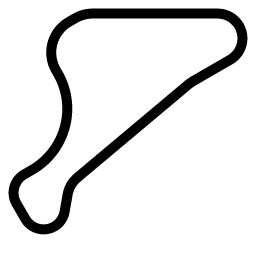
\includegraphics[width=1.2in]{CG-Speedway}}
% \label{fig_second_case}} 
\caption{FSMDriver test tracks.} 
\label{fig:tracks} 
\end{figure} 



The first track considered is B-Speedway
When racing in oval tracks, particularly in , the FSMDriver outperforms 
some of the controllers provided by the TORCS distribution. The FSMDriver raced 
against considered average drivers and performed very well, winning even if it 
started behind them.

\begin{table}[h]
\renewcommand{\arraystretch}{1.3}
\caption{3 Laps Race in B-Speedway}
\label{table_1}
\centering
\begin{tabular}{c||c||c||c}
\hline
\bfseries Driver & \bfseries Total Time & \bfseries Damage & \bfseries Top Speed \\ 
\hline
\hline FSMDriver & 02:34:95 & 1 & 299 \\ 
\hline Berniw 10 & 02:40:59 & 8 & 282 \\ 
\hline 
\end{tabular}
\end{table}

\begin{table}[h]
\renewcommand{\arraystretch}{1.3}
\caption{3 Laps Race in B-Speedway}
\label{table_2}
\centering
\begin{tabular}{c||c||c||c}
\hline
\bfseries Driver & \bfseries Total Time & \bfseries Damage & \bfseries Top Speed \\ 
\hline
\hline FSMDriver & 02:34:88 & 1 & 299 \\ 
\hline Olethros 10 & 02:47:38 & 5 & 282 \\ 
\hline 
\end{tabular}
\end{table}

\begin{table}[h]
\renewcommand{\arraystretch}{1.3}
\caption{3 Laps Race in B-Speedway}
\label{table_3}
\centering
\begin{tabular}{c||c||c||c}
\hline
\bfseries Driver & \bfseries Total Time & \bfseries Damage & \bfseries Top Speed \\ 
\hline
\hline FSMDriver & 02:34:90 & 1 & 299 \\ 
\hline Illaw 10 & 02:39:82 & 0 & 283 \\ 
\hline 
\end{tabular}
\end{table}



In the other hand, when facing considered good drivers the controller was defeated. However, if more than one driver race against FSMDriver at the same time, it will benefit from the crashes and finish in better positions.

\begin{table}[h]
\renewcommand{\arraystretch}{1.3}
\caption{3 Laps Race in CG-Speedway 1}
\label{table_4}
\centering
\begin{tabular}{c||c||c||c}
\hline  \bfseries Driver & \bfseries Total Time & \bfseries  Damage & \bfseries Top Speed \\ 
\hline Inferno 3 & 02:30:92 & 0 & 300 \\ 
\hline Olethros 3 & 02:33:19 & 210 & 317 \\  
\hline bt 3 & 02:33:23 & 0 & 303 \\  
\hline FSMDriver & 02:33:30 & 315 & 309 \\  
\hline Berniw 3 & 02:39:52 & 0 & 312 \\
\hline Iliaw 3 & 02:40:62 & 1635 0 & 314 \\
\hline Tita 3 & 02:52:15 & 1794 & 300 \\
\hline 
\end{tabular}
\end{table} 


The damage taken can be significantly reduced by implementing an enemy avoidance and overtaking behavior,

Although, when it comes to road tracks, especially the ones filled with critical curves combinations, the controller faces several problems at staying between the track boundaries. These troubles are mainly caused by entering curves with high speed values, fact that reinforces the idea of an approaching curve state, to deal with speed reductions and angle corrections. In addition, the constants used in transition process do not represent the optimal values for that role, an evolutionary method needs to be implemented in order to achieve those values. Moreover, oval tracks barely requires a state transition, in the overwhelming majority of time the car fits in the straight state. This lack of transitions and accentuated curves improves significantly the gain in performance.

\subsection{Parameter changing}
At the beginning those parameter were imported from the Simple Driver provided by Danielle Loiacono, as expected they did not lead to satisfying results when compared to the drivers available in TORCS.

For initial improvements the transition parameters have been chosen. 


\begin{table}[h]
\renewcommand{\arraystretch}{1.3}
\caption{Parameters Used for Enhancement}
\label{parameter_table}
\centering
\begin{tabular}{c||c||c||c}
\hline \bfseries $p$ &\bfseries $p_0$ &\bfseries $ p_{max}$ &\bfseries $\Delta p$ \\
\hline
\hline MSD & $20$ & $200$ & $5$ \\ 
\hline LE & $-1$ & $-0.8$ & $0.1$ \\ 
\hline RE & $1$ & $0.8$ & $-0.1$ \\ 
\hline ST & $30$ & $300$ & $10$ \\ 
\hline 
\end{tabular} 
\end{table}

In the end 8658 combinations were generated and properly tested in \textit{CG Speedway 1}
for three laps. The best result generated used the following parameters: MAX\_SPEED\_DIST: $20$, LEFT\_EDGE: $-0.8$, RIGHT\_EDGE: $1$, STUCK\_TICKS: $110$.

\begin{table}[h]
\renewcommand{\arraystretch}{1.3}
\caption{Comparison Among Lupo Bianco, who achieved the best results in CG Speedway 1, Berniw 3 and The FSMDriver}
\label{results_table}
\centering

\begin{tabular}{c||c||c||c}
\hline \bfseries Driver &\bfseries Total Time &\bfseries Best Lap &\bfseries Top Speed \\
\hline
\hline Lupo Bianco & 01:50:12 & 00:35:22 & 262 \\
\hline Berniw 3 & 02:07:28 & 00:40:97 & 247 \\ 
\hline FSMDriver & 02:34:49 & 00:50:12 & 242 \\ 
\hline 
\end{tabular}
\end{table}
This approach demands a lot of time and space since all combinations are generated and executed. For future evolutions a more robust method, like genetic algorithm or neural networks needs to be applied in order to provide reliable results.
